% !TeX root = ../build/main.tex

Protocol implementation involves realization of the protocol building blocks as well as providing means of data communication between them. Building blocks are placed at the following locations, which correspond to protocol participants:

\begin{itemize}%[label=$\bullet$]
	\item User software.
	\item License Provider software.
	\item Service Provider software.
	\item License contract.
\end{itemize}

\begin{flushleft}
	Data communication between protocol participants is realized in the following modes:
\end{flushleft}

\begin{itemize}%[label=$\bullet$]
	\item Calling a contract state changing method.
	\item Calling a contract state querying method (not modifying the contract state).
	\item Storing data directly in blockchain.
	\item Retrieving data from blockchain.
	\item Delegating ZK proof calculation.
	\item Calling off-chain.
\end{itemize}

\begin{flushleft}
	The following diagram in Figure~\ref{fig:implementation} illustrates the interaction between protocol participants and indicates the communication means used.
\end{flushleft}

\begin{figure}[h!]
	\centering
	\fbox{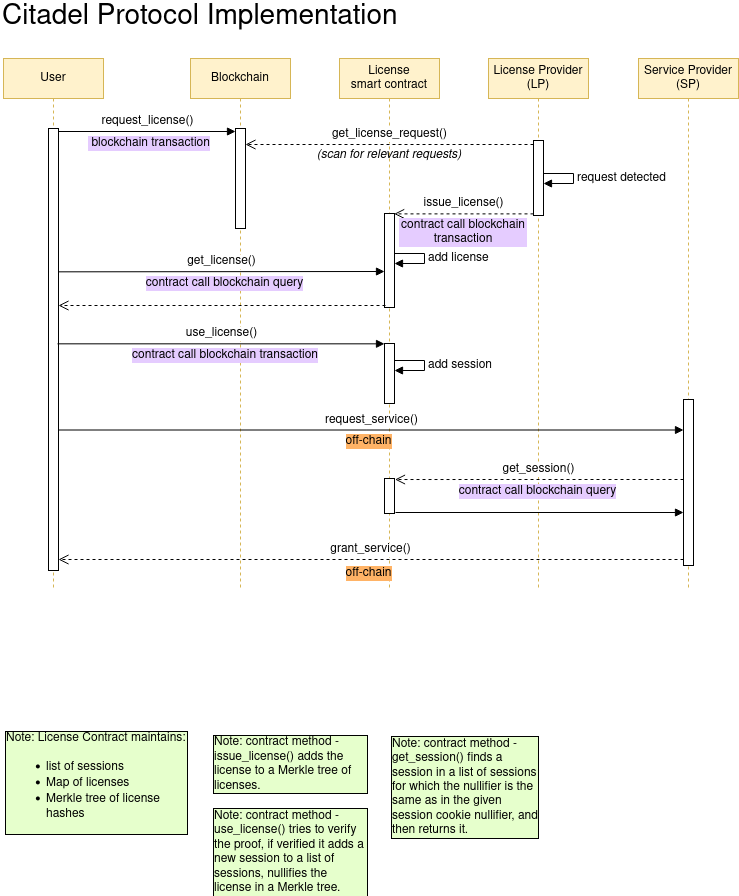
\includegraphics[width=380pt,draft=false]{\figs/implementation.png}}
	\caption{Interaction between protocol participants.}
	\label{fig:implementation}
\end{figure}

On the diagram, we can see various communication modes being used. Initially, the user submits to the blockchain a transaction which contains request as a payload. Subsequently, the License Provider, which continuously scans the blockchain, detects transactions containing requests and filters out requests which are addressed to it. The License Provider can obtain requests via other routes as well, for example via http or email, passing requests on the blockchain is only one of many possible ways of submitting a request, one that has the advantage of passing a payment along with the request. Once the License Provider gets a hold of a request, it can perform appropriate verification, and upon successful verification, it can issue a license. Issuing a license involves a smart contract transaction call. Smart contract transaction call is a blockchain transaction, yet to not confuse the reader, we show it on the diagram with details of blockchain involvement omitted. The user obtains licenses via a contract query. For privacy reasons, the user obtains a bulk of licenses not pertaining exclusively to her and filters it out by herself. To economize the volume of data transfers, block-height range is passed to allow for tranfer of a subset of available records. All modes of communication used so far were on-chain. Communication between the user and the Service Provider, on the other hand, is off-chain. When the Service Provider wants to establish a session, it calls a contract to obtain a session for the given session id.

The diagram illustrates the following flow of data and interactions between participants:

\begin{itemize}%[label=$\bullet$]
	\item User submits request to a License Provider by issuing a blockchain transaction.
	\item License Provider scans the blockchain and obtains the request.
	\item License Provider, upon necessary verification, issues a license.
	\item License Provider sends license to the License Contract via a smart contract call transaction.
	\item User obtains licenses for a given block-height range.
	\item User filters out licenses addressed to her/him.
	\item User calculates a proof (the proof calculation might be delegated).
	\item User calls \textit{use-license} to redeem a license, via a smart contract call.
	\item License Contract attempts to verify the proof and, if verified, adds a new session to a list of sessions.
	\item User requests a service from a Service Provider (off-chain).
	\item Service Provider asks contract for a session.
	\item Service Provider grants service to the user (off-chain).
\end{itemize}
